\subsection{Five Parameter Solar Cell Model}\label{subsec:five_parameter_solar_cell_model}

\begin{figure}[h]
    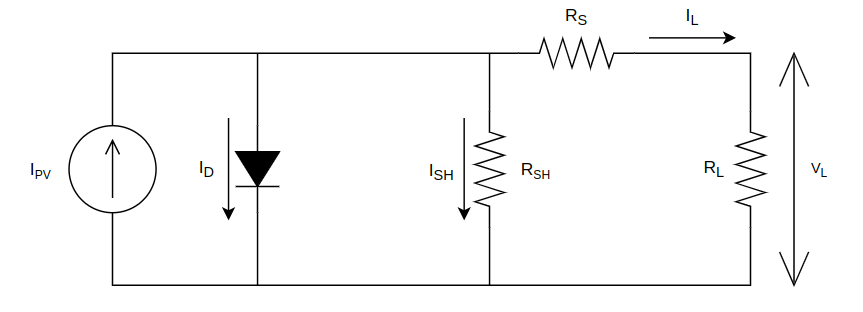
\includegraphics[width=\textwidth]{solar_cell_five_parameter_model.png}
    \caption{Five Parameter, or Full Single Diode Model of a Solar Cell}
    \label{fig:single_diode_model_with_resistances}
\end{figure}

The most common model for solar cells is the five parameter solar cell model,
shown in \autoref{fig:single_diode_model_with_resistances}. This is the complete
form of the single diode model discussed in the previous section,
\autoref{subsec:three_parameter_solar_cell_model}. There are two added
components/parameters: a \acf{RS} and \acf{RSH}, whose primary roles are to
alter the shape of the knee-bend in the I-V curve. As such, this model improves
upon the main flaw of the three parameter solar cell model, that of poorly
predicting points clustering around the maximum power point.

In the following, we discuss the two added parameters and their specific effects
on the model.


\subsubsection{Shunt Resistance}\label{subsubsec:five_param_shunt_resistance}

\begin{figure}[h]
    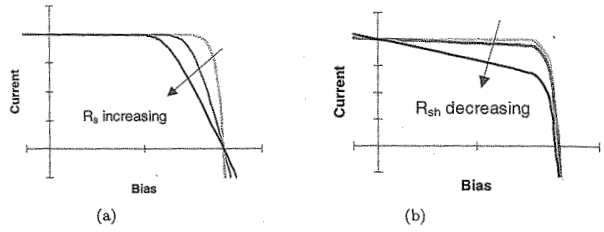
\includegraphics[width=\textwidth]{series_shunt_resistance.png}
    \caption{Effect of Series (a) and Shunt Resistance (b) on \ac{I-V} Curve}
    \label{fig:series_shunt_resistance}
\end{figure}

As shown in \autoref{fig:series_shunt_resistance} (b) from Nelson~\cite{nelson},
as the \acf{RSH} decreases, the top of the knee-bend of the \acf{I-V} curve will
be forced down. At low values of \ac{RSH} (on the order of $10$ $\si{\ohm}$),
the knee-bend will be pushed down so much that the curve becomes a straight
line. At high values of \ac{RSH}, (on the order of $100$ $\si{\ohm}$), the curve
converges to some fixed maximum bend constrained by other parameters of the
model. This relationship is generally considered logarithmic.

The \acf{ISH} can be added to the simple form of the model as a new term as
shown in \autoref{eq:cell_output_current_3}. Assuming that the \acf{RS} is
negligible ($0$), we can determine that \ac{ISH} is a function of the \ac{RSH}
and the \acf{VL}, as shown in \autoref{eq:cell_output_current_4}.

\begin{equation}
    I_L = I_{PV} - I_D - I_{SH}
    \equnit{\si{\ampere}}
    \label{eq:cell_output_current_3}
\end{equation}

\begin{equation}
    I_L = I_{PV} - I_D - \frac{V_L}{R_{SH}}
    \equnit{\si{\ampere}}
    \label{eq:cell_output_current_4}
\end{equation}


\subsubsection{Series Resistance}\label{subsubsec:five_param_series_resistance}

The \acf{RS} forces the knee-bend of the \ac{I-V} curve to the left or right, as
opposed to up and down for \ac{RSH}. As \ac{RS} increases, more current is
consumed across the lumped resistance before reaching the terminals of the solar
cell, reducing the expected current in the curve as shown in
\autoref{fig:series_shunt_resistance} (a). At high values of \ac{RS}, the curve
likewise becomes a straight line.

The \ac{RS} term impacts the consumers of the five parameter solar cell model;
namely the \ac{ID} and the \ac{RSH} terms. A visualization of this is shown as
\autoref{fig:current_junction}.

\begin{figure}[!htbp]
    \centering
    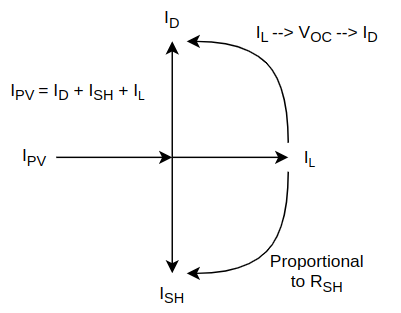
\includegraphics[width=0.6\textwidth]{cell_kirchoff_current_junction.png}
    \caption{Current Flow Junction of Five Parameter Model Solar Cell}
    \label{fig:current_junction}
\end{figure}

Revisiting \autoref{eq:cell_dark_current_1}, we know that the dark current
depends on \acf{VL} generated by \acf{IL} flowing through equivalent \acf{RL} connected at the cell
terminals. This allows us to reformulate the dark current equation as
\autoref{eq:cell_dark_current_2}. Here, we add the voltage drop across the
lumped series resistance summed with the \ac{VL} to represent the
total voltage expected by the dark current model.

\begin{equation}
    I_D = I_0[\exp(\frac{V_L + I_L R_S}{V_T}) - 1]
    \equnit{\si{\ampere}}
    \label{eq:cell_dark_current_2}
\end{equation}

We can likewise use the voltage drop to update the \ac{ISH} term, shown
in \autoref{eq:cell_shunt_current}.

\begin{equation}
    I_{SH} = \frac{V_L + I_L R_S}{R_{SH}}
    \equnit{\si{\ampere}}
    \label{eq:cell_shunt_current}
\end{equation}

Combining these two effects, we form \autoref{eq:cell_output_current_5}.

\begin{equation}
    I_{L} =  I_{PV} - I_0[\exp(\frac{V_L + I_L R_S}{V_T}) - 1] - \frac{V_L + I_L R_S}{R_{SH}}
    \equnit{\si{\ampere}}
    \label{eq:cell_output_current_5}
\end{equation}

We note that this model is an implicit function and cannot easily (or prettily)
move all the \ac{IL} terms to the left side of the equation. As such, for these
types of problems, we will develop and use iterative solvers to determine
\ac{IL} for a given set of input parameters (\ac{RS}, \ac{G}, \ac{VL}, etc).
Iterative solvers involve starting with a guess for the output parameter (in
this case \ac{IL}) and attempt to improve upon that guess such that each side is
equal to each other or within some tolerance to each other. An in depth
discussion on how these solvers were implemented for this model and variants of
this model can be found in \autoref{appendix:iterative_solvers}.

\todo[inline]{Augment appendix note with reference to
\ref{subsubsec:modeling_solar_cell_datasets}. Relegate appendix note to discussion
about iterative solvers and steps to build iterative solver (Desmos -\> MATLAB -\>
Python).}


\subsubsection{Photocurrent as a Function of Parasitics}\label{subsubsec:photocurrent_shunt_series_relation}

An interesting addition to the five parameter cell model is presented by Cubas
et al~\cites{cubas_et_al,cubas_et_al_2}: they observe that
\autoref{eq:cell_output_current_5} in short circuit conditions results in
\autoref{eq:cell_short_circuit_current_6}.

\begin{equation}
    I_{SC} = I_{PV} - I_0[\exp(\frac{I_{SC} R_S}{V_T}) - 1] - \frac{I_{SC} R_S}{R_{SH}}
    \equnit{\si{\ampere}}
    \label{eq:cell_short_circuit_current_6}
\end{equation}

In their analysis of measurements taken across a broad spectrum of reference
solar cells, represented in \autoref{table:dark_current_reference}, the dark
current at short circuit conditions were well less than a single milliampere, an
insignificant fraction of the total operating current. From this observation
Cubas et al. rewrites the above expression to get the photocurrent as a function
of \ac{ISC} and a ratio of \ac{RS} and \ac{RSH}, shown in
\autoref{eq:cell_photocurrent_3}.

\begin{equation}
    I_{PV} = I_{SC}\frac{R_S + R_{SH}}{R_{SH}}
    \equnit{\si{\ampere}}
    \label{eq:cell_photocurrent_3}
\end{equation}

\begin{table}[h!]
    \begin{tabularx}{\textwidth}{
        | >{\raggedright\arraybackslash}X
        | >{\raggedright\arraybackslash}X
        | >{\raggedright\arraybackslash}X
        | >{\raggedright\arraybackslash}X
        | >{\raggedright\arraybackslash}X | }
        \hline
        Reference & Cell Type & \ac{ISC} (A) & $I_0[e^{\frac{I_{SC} R_S}{V_T}} -
        1]$ (A) & \ac{ID} / \ac{ISC} \\ \hline \hline
        Kennerud, 1969  & CdS   & 0.8040 & 1.56E-5 & 1.94E-5 \\ \hline
        Charles, 1981   & BSC   & 0.1023 & 2.21E-8 & 2.16E-7 \\ \hline
        Charles, 1981   & GSC   & 0.5610 & 1.01E-5 & 1.80E-5 \\ \hline
        Lo Brano, 2010  & Q6LM  & 7.6650 & 1.42E-9 & 1.85E-10 \\ \hline
    \end{tabularx}
    \caption{Dark Current Ratios for Various Reference Cells~\cite{cubas_et_al}}
    \label{table:dark_current_reference}
\end{table}

However, a cursory evaluation of the parameter space (\ac{VOC}, \ac{ISC},
\ac{G}, \ac{TC}, \ac{RS}, \ac{N}) reveals that the assumption that the dark
current is negligible breaks down when a subset of the following conditions
occur:

\begin{itemize}
    \item the \acf{VOC} becomes very small,
    \item the \acf{ISC} becomes very large,
    \item and the \acf{RS} becomes relatively large for some
    combination of \ac{VOC} and \ac{ISC}.
\end{itemize}

Is it to be noted that these parameters are tightly coupled, and therefore the
language specifying a parameter space upon which this term should be used
remains imprecise. We also note that \ac{TC} and \ac{N} when increased slightly
tighten the viable parameter space.

However, when considering a specific solar cell that is \textit{appropriate}
(e.g.\ it contains \ac{STC} defined parameters \ac{VOC} and \ac{ISC} with an
measured \ac{RS} that results in negligible \ac{ID}), this term remains
negligible unless the cell is exposed to (1) high temperatures or (2) high
intensity light, two conditions that tend to come hand in hand. These conditions
tend to only be experienced by concentrator photovoltaics and are highly
unlikely to be reached by normal solar cells.

We will observe later in \autoref{subsec:eval_solar_cell_models} that with our
dataset of Maxeon Gen III Bin Le1 solar cells, the vast majority of estimated
series resistance is well below $0.08 \si{\ohm}$, which results in dark currents
less than a m\si{\ampere}. This means that this modification (assuming it
improves the accuracy of the model), is well suited for our solar cells.

Incorporating this revision, we arrive at
\autoref{eq:cell_short_circuit_current_7}.

\begin{equation}
    I_L = I_{SC}\frac{R_S + R_{SH}}{R_{SH}} - I_0[\exp(\frac{V_L + I_L R_S}{V_T}) - 1] - \frac{V_L + I_L R_S}{R_{SH}}
    \equnit{\si{\ampere}}
    \label{eq:cell_short_circuit_current_7}
\end{equation}

\todo[inline]{See \url{https://www.desmos.com/calculator/nniw0mha2k} to play
around with the revised dark current model. Add as a figure later on compared to
experimental data.}


\subsubsection{Parisitics as a Function of Irrad., Temp.}\label{subsubsec:rsh_rs_dependence}

Throughout this discussion, we introduced the notion of shunt and series
resistance as internal parasitics. However, we did not explore whether these
`internal parameters' are themselves affected by external conditions such as
irradiance and temperature.

A comprehensive review and experimental paper from Fébba et
al~\cite{febba_et_al} performed experiments on solar cells to evaluate the
effect of temperature and irradiance on shunt and series resistance, controlling
for the two independent variables in ranges of $25\si{\celsius}$ to
$55\si{\celsius}$ and $600\si{\watt/\meter^2}$ to $1000\si{\watt/\meter^2}$,
respectively. Four figures,
\autoref{fig:febba_shunt_resistance_and_temperature}~-~\autoref{fig:febba_series_resistance_and_irradiance}
are shown below to illustrate the following assertions.

For \acf{RSH}, they observed the following trends:

\begin{itemize}
    \item as temperature increases, the \ac{RSH} exponentially decays,
    \item and as irradiance increases, the \ac{RSH} linearly decreases.
\end{itemize}

For \ac{RS}, they observed the following trends:

\begin{itemize}
    \item as temperature increases, the \ac{RS} exponentially decays,
    \item and as irradiance increases, the \ac{RS} linearly increases.
\end{itemize}

\begin{figure}[!htbp]
    \centering
    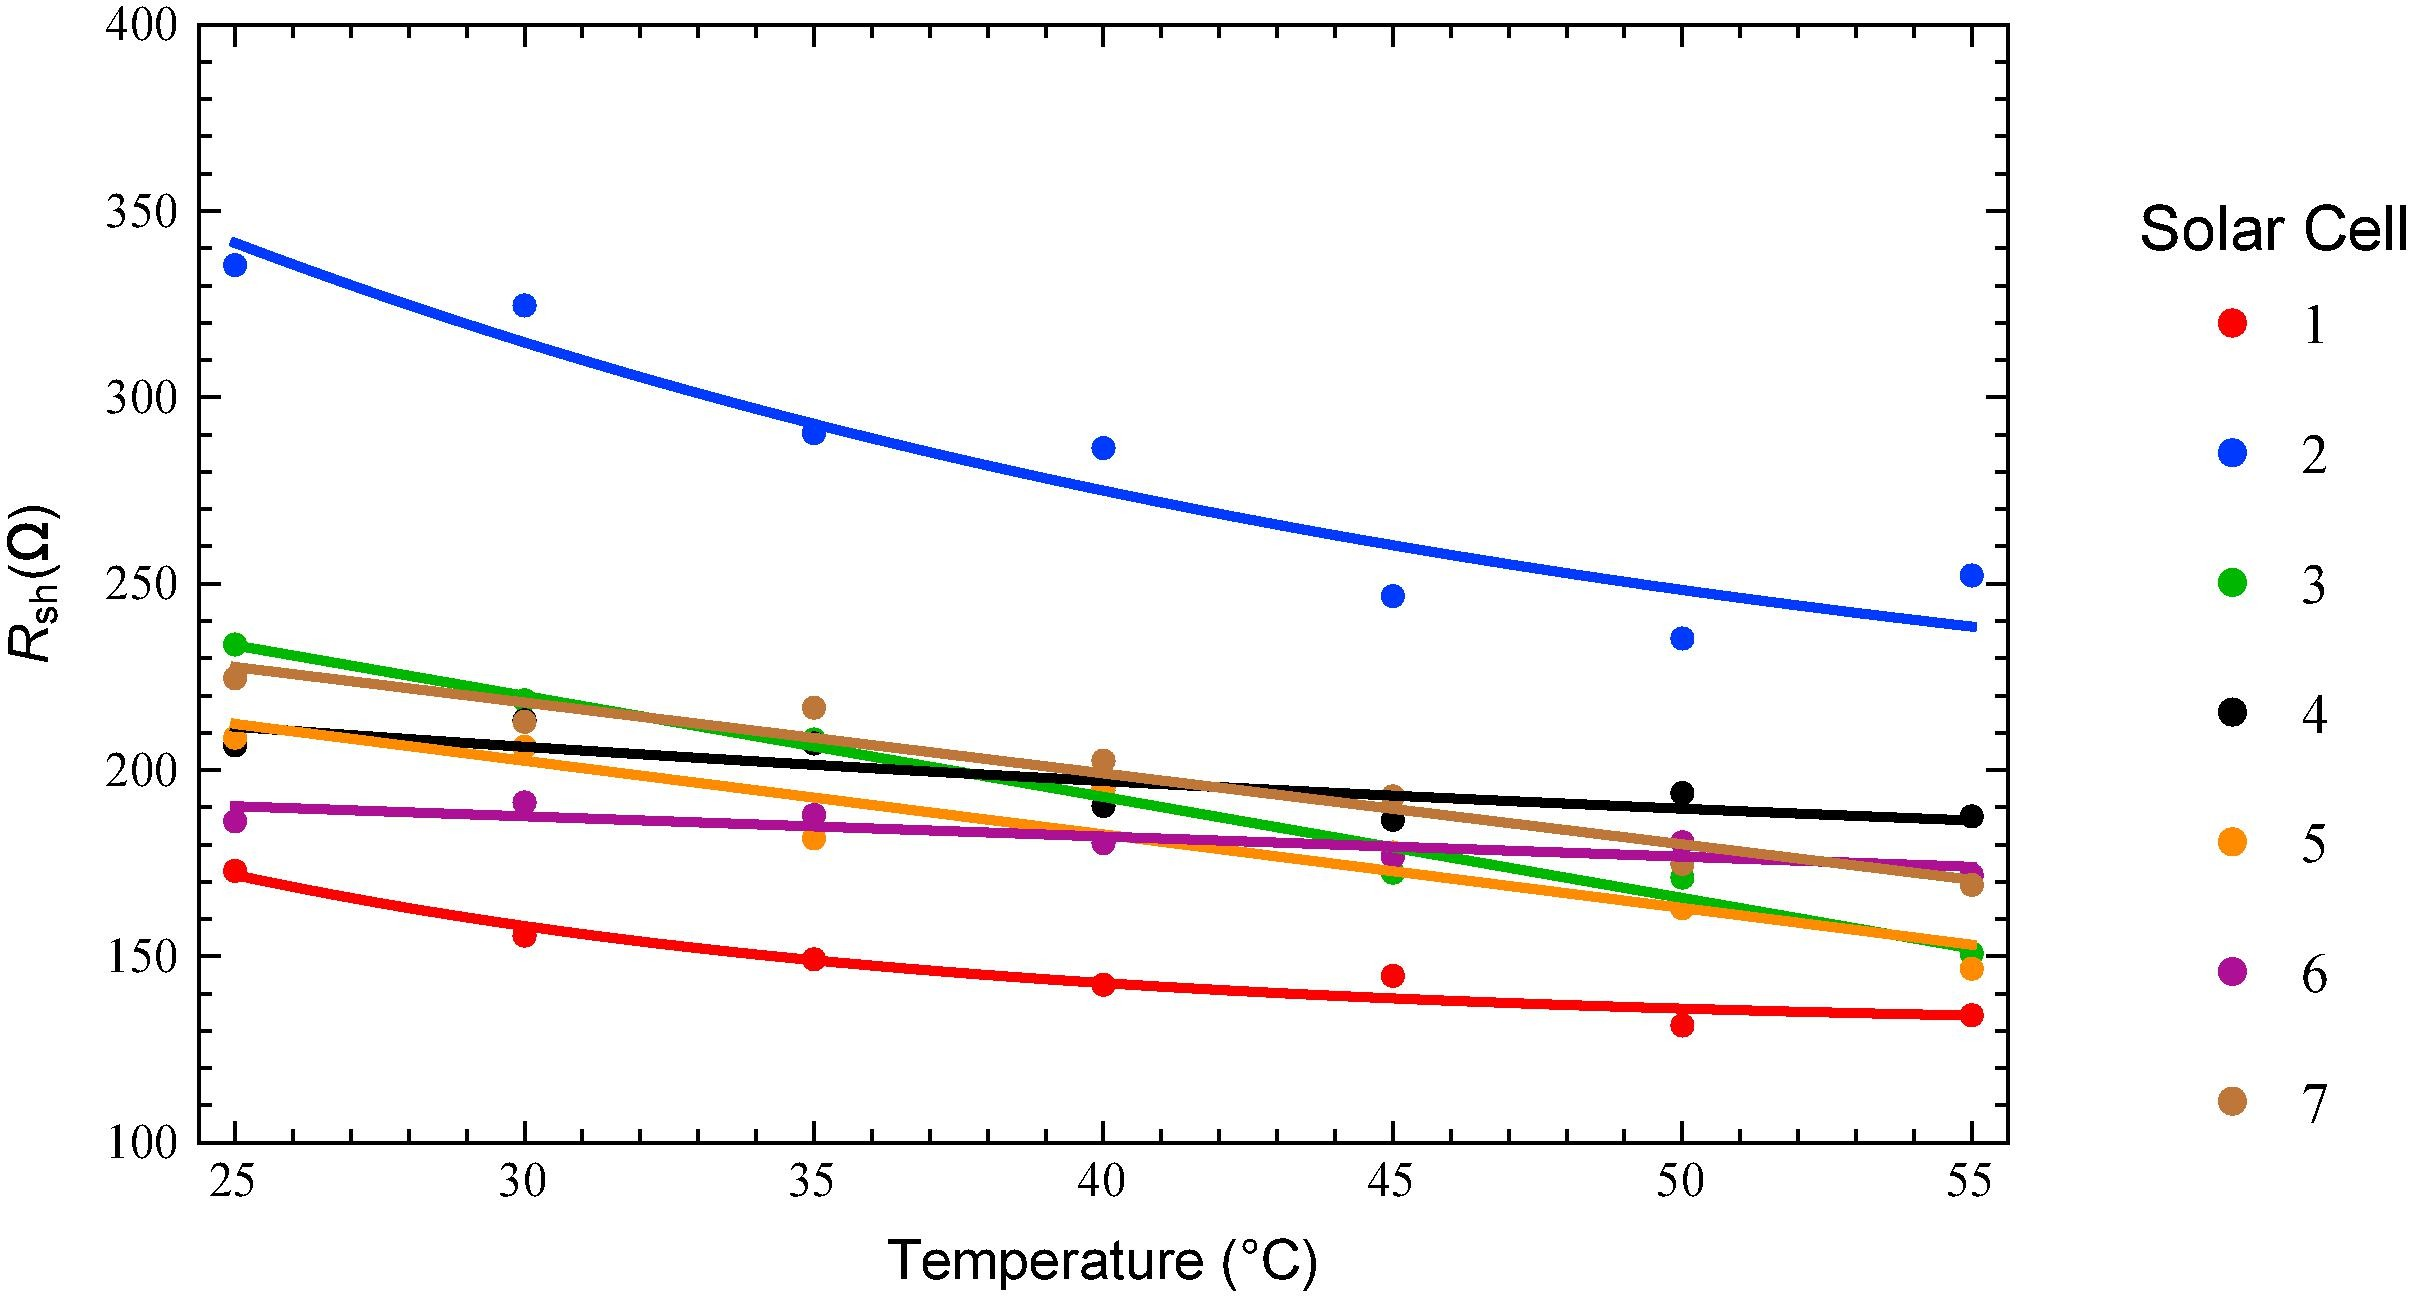
\includegraphics[width=\textwidth]{febba_shunt_resistance_and_temperature.jpg}
    \caption{Shunt Resistance vs Temperature~\cite{febba_et_al}}
    \label{fig:febba_shunt_resistance_and_temperature}
\end{figure}

\begin{figure}[!htbp]
    \centering
    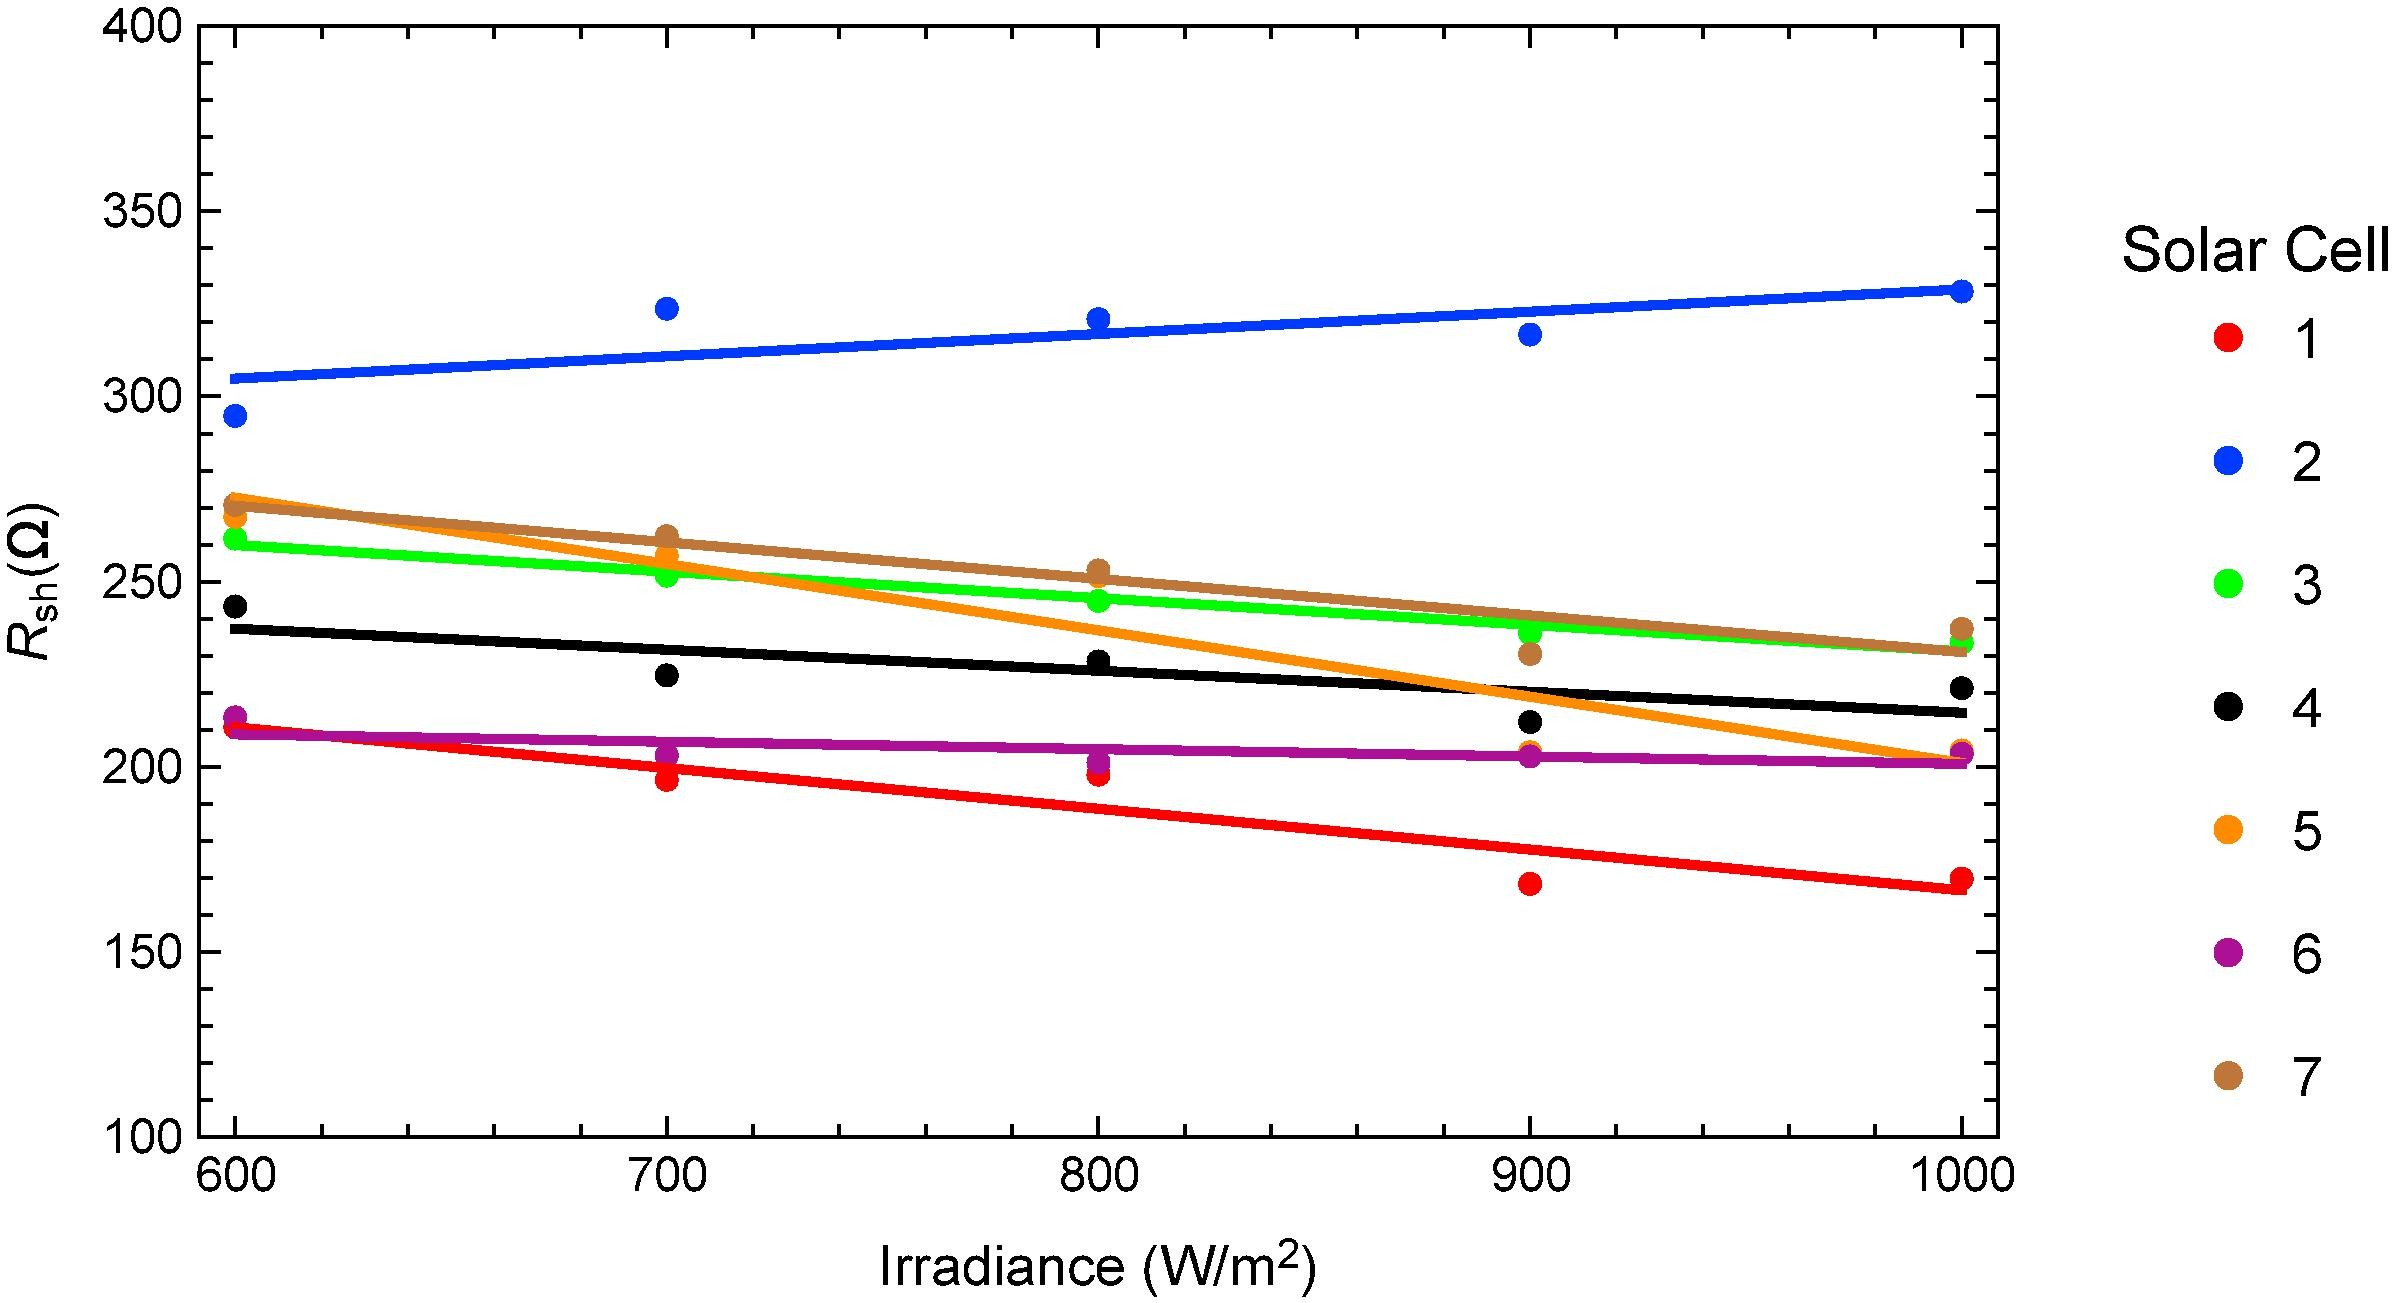
\includegraphics[width=\textwidth]{febba_shunt_resistance_and_irradiance.jpg}
    \caption{Shunt Resistance vs Irradiance~\cite{febba_et_al}}
    \label{fig:febba_shunt_resistance_and_irradiance}
\end{figure}

\begin{figure}[!htbp]
    \centering
    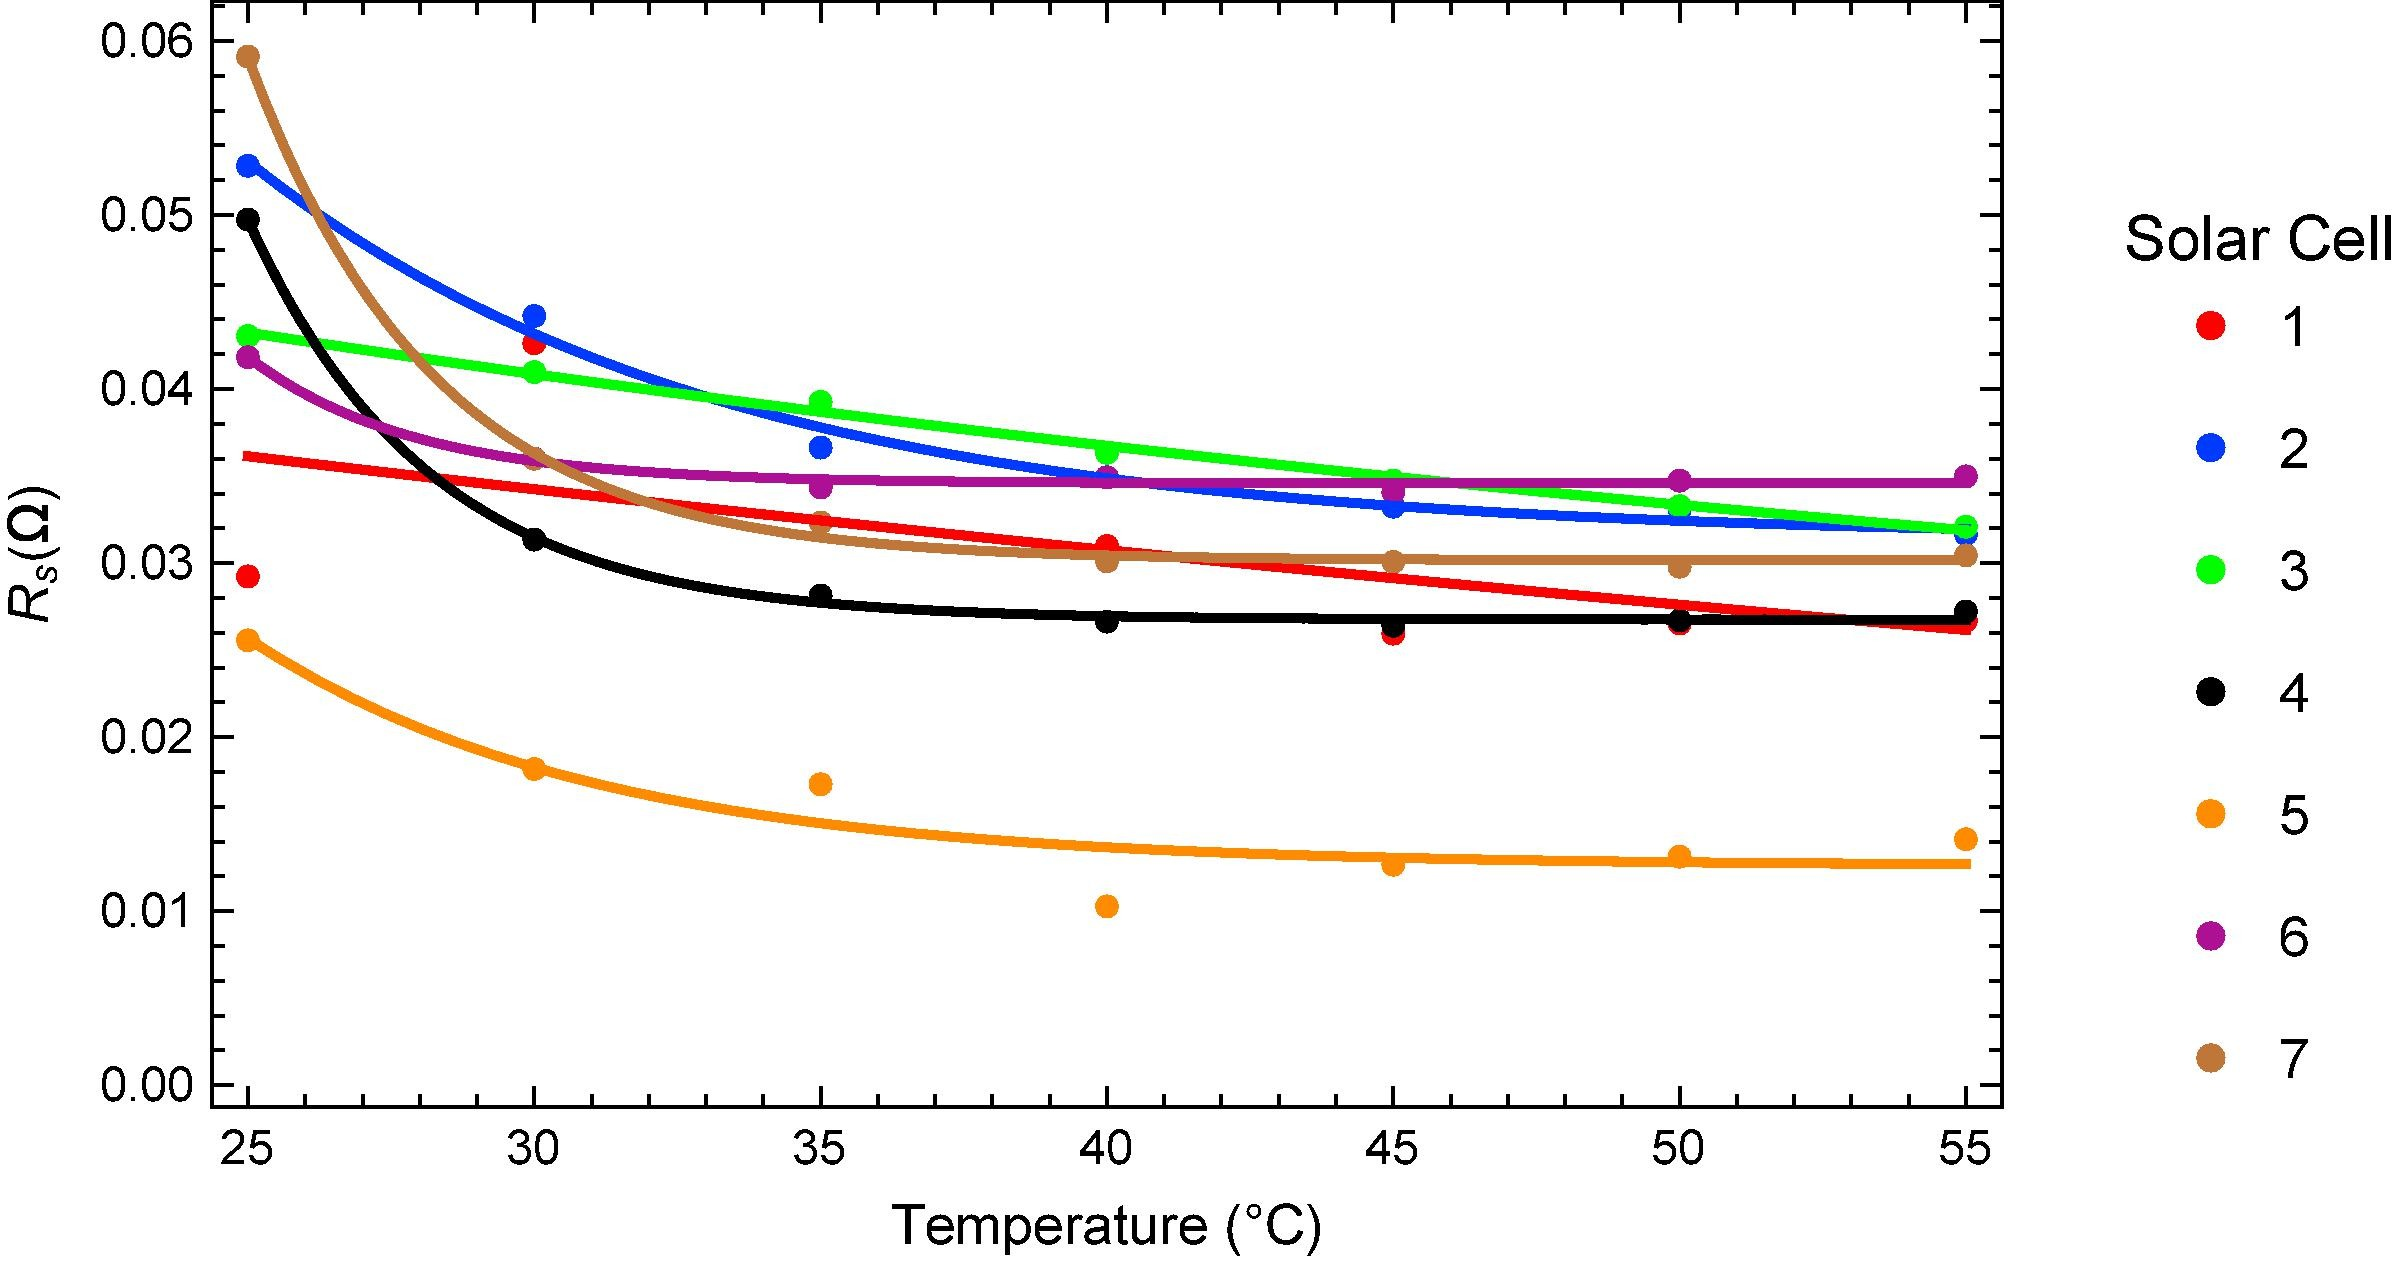
\includegraphics[width=\textwidth]{febba_series_resistance_and_temperature.jpg}
    \caption{Series Resistance vs Temperature~\cite{febba_et_al}}
    \label{fig:febba_series_resistance_and_temperature}
\end{figure}

\begin{figure}[!htbp]
    \centering
    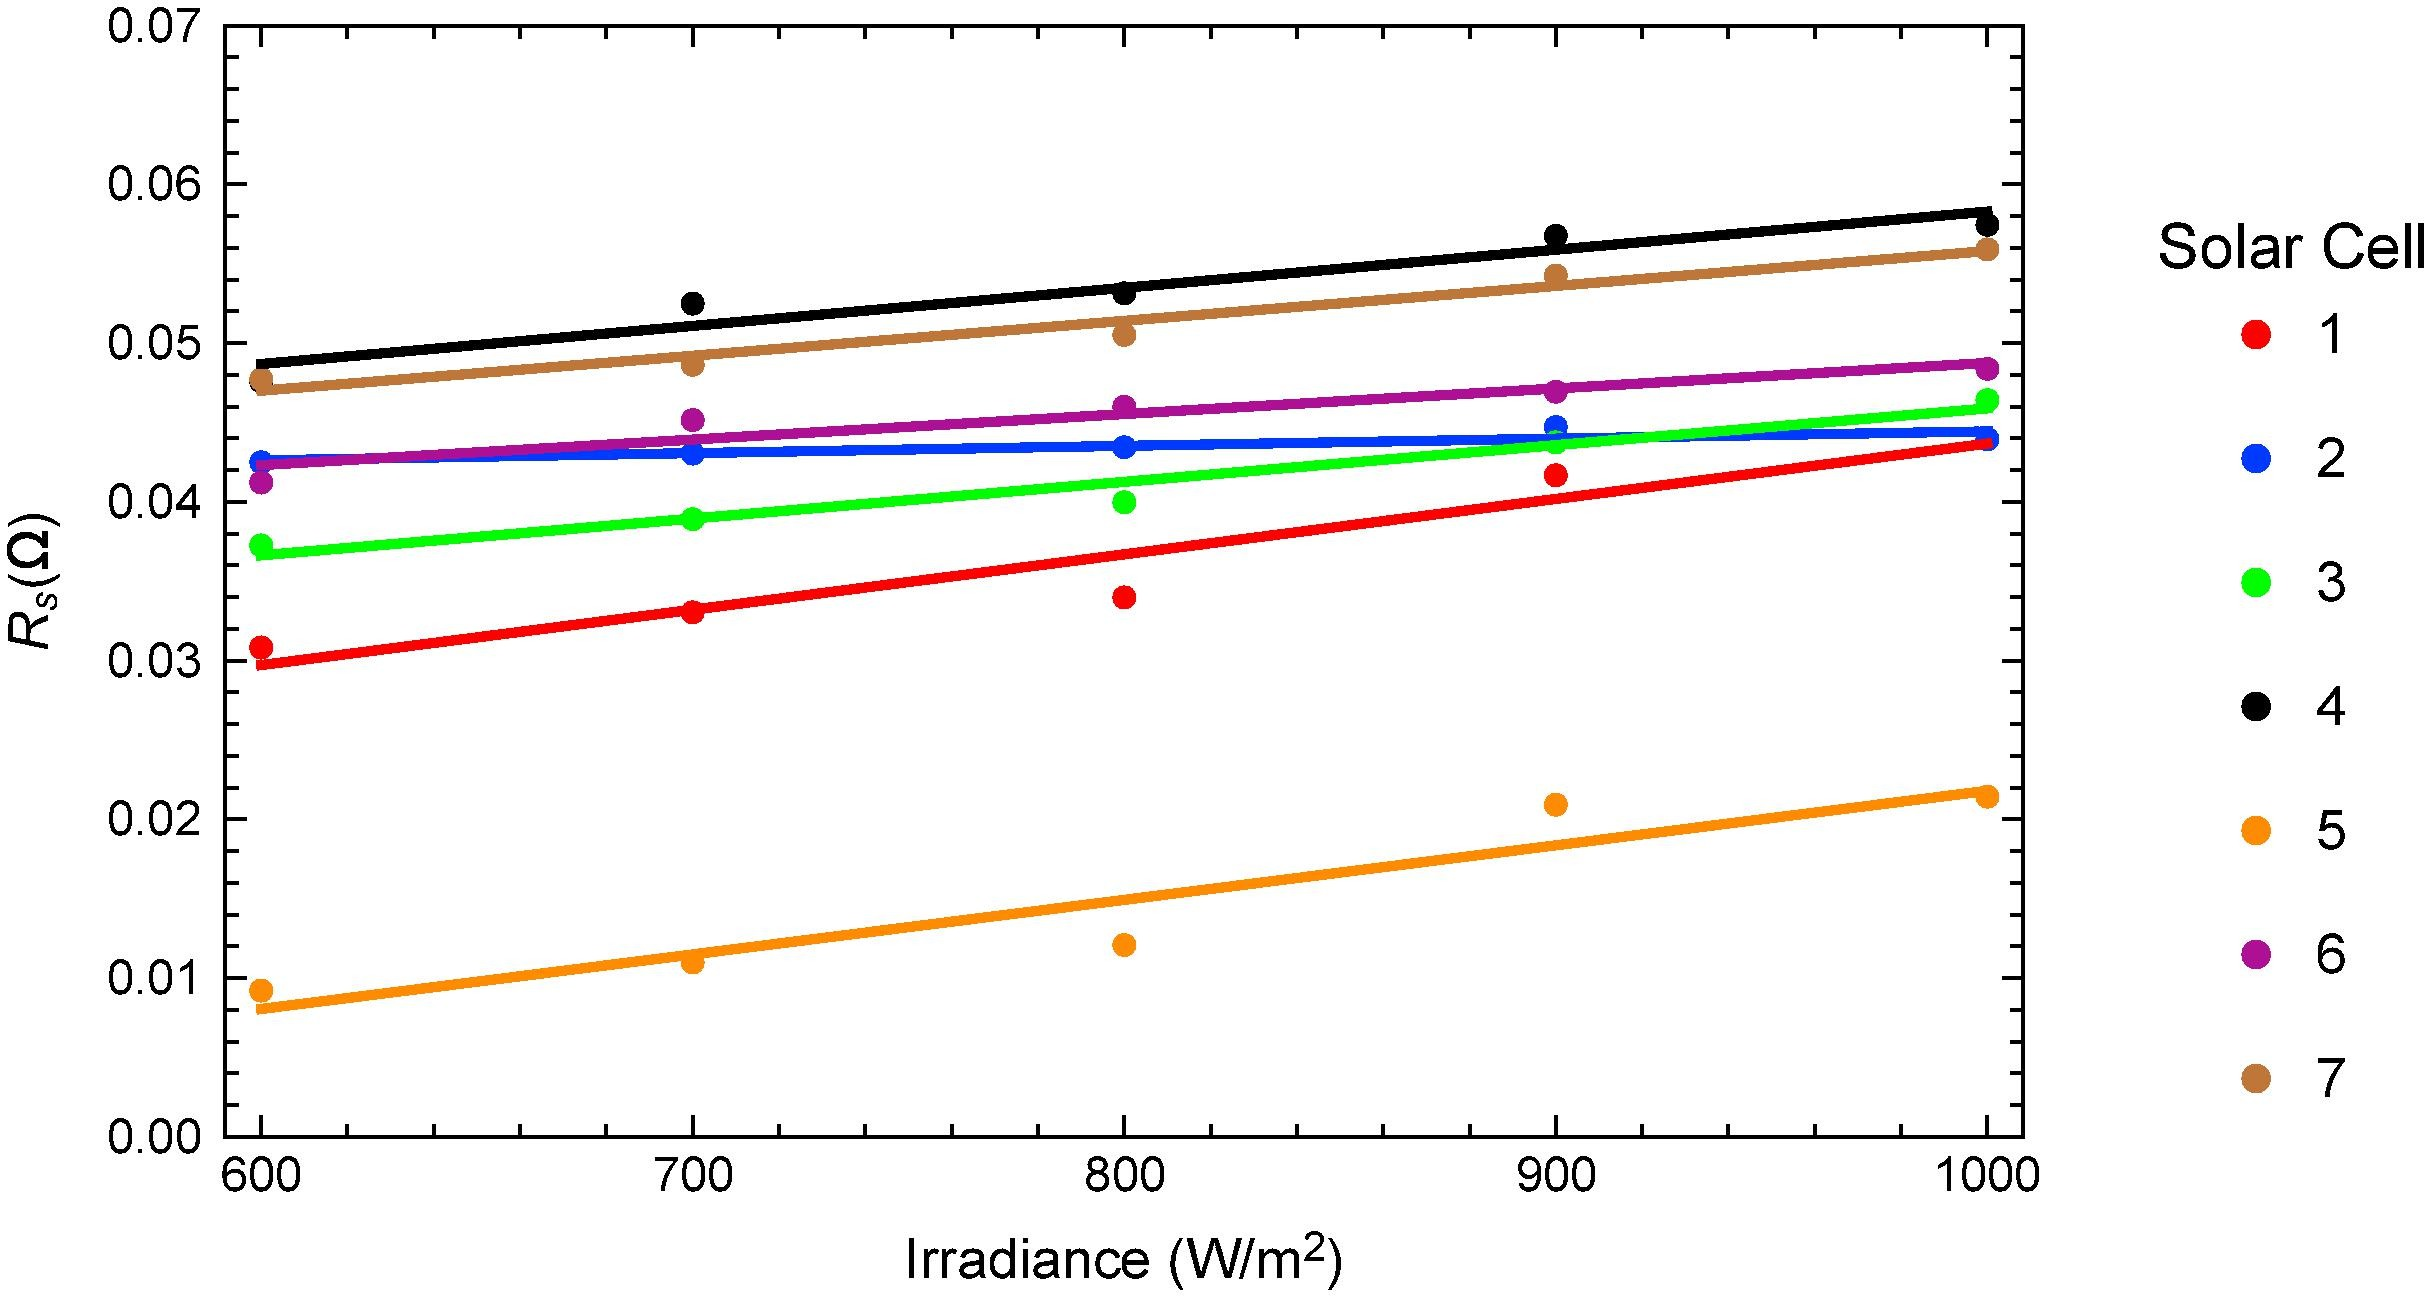
\includegraphics[width=\textwidth]{febba_series_resistance_and_irradiance.jpg}
    \caption{Series Resistance vs Irradiance~\cite{febba_et_al}}
    \label{fig:febba_series_resistance_and_irradiance}
\end{figure}

Fébba et al. did not posit a revised model of the either resistance term
(although they did provide explanations on why the trends were reasonable), but
Baig et al.~\cite{baig_et_al} and MacAlpine et
Brandemuehl~\cite{macalpine_et_brandemuehl} introduced a variant of
\autoref{eq:series_resistance_1} that uses a \ac{ZETA}.

\begin{equation}
    R_S = R_{S,ref} \exp(\zeta [T_{C,ref} - T_C])
    \equnit{\si{\ohm}}
    \label{eq:series_resistance_1}
\end{equation}

We extend Fébba et al~\cite{febba_et_al}'s results to generate
\autoref{eq:series_resistance_2}, adding a \ac{ETA}, applied to
\autoref{eq:series_resistance_1}.

\begin{equation}
    R_S = R_{S,ref} \exp(\zeta [T_{C,ref} - T_C])[1 + \eta(G_{ref} - G)]
    \equnit{\si{\ohm}}
    \label{eq:series_resistance_2}
\end{equation}

We also propose \autoref{eq:shunt_resistance} to model the shunt
resistance, with \ac{KAPPA} and \ac{IOTA}.

\begin{equation}
    R_{SH} = R_{SH,ref} \exp(\kappa [T_{C,ref} - T_C])[1 + \iota [G_{ref} - G]]
    \equnit{\si{\ohm}}
    \label{eq:shunt_resistance}
\end{equation}

\autoref{eq:series_resistance_2} and \autoref{eq:shunt_resistance}'s
coefficients are not provided by the manufacturer, so they will have to be
estimated. We'll look at ways to measure series and shunt resistance in
\autoref{subsubsec:experimental_extraction_of_cell_parameters}, and how to take
advantage of our test setup to measure the coefficients. Additionally, we'll
attempt to replicate Fébba et al's work on a broader scale, with a temperature
and irradiance range of ($0\si{\celsius}$ to $100\si{\celsius}$
and $0\si{\watt/\meter^2}$ to $1000\si{\watt/\meter^2}$, respectively).


\subsubsection{Non Uniform Series Resistance}\label{subsubsec:nonuniform_series_resistance}

As an aside to this thesis, we note that the solar cell models described assume
that the cell is uniform in composition and thus can represent the series
resistance as a lumped resistance. In actuality, the cell is a two (actually
three, but for all intents and purposes the thickness is irrelevant in terms of
affecting the series resistance -although it may affect the shunt resistance)
dimensional network of resistors and diodes
(\autoref{fig:cell_with_varying_series_resistance}).

\begin{figure}[!htbp]
    \centering
    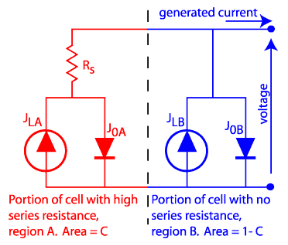
\includegraphics[width=0.6\textwidth]{cell_with_varying_series_resistance.png}
    \caption{Solar Cell With Varying Series Resistances~\cite{pveducation_measurement_of_series_resistance}}
    \label{fig:cell_with_varying_series_resistance}
\end{figure}

This series resistance non uniformity becomes more important to the
resultant \ac{I-V} curve in low light conditions. Under uniform, bright
conditions, current from the photovoltaic effect is generated evenly and
conducts to the contacts regardless of the resistance along the paths. In the
dark, any current that has to flow through the cell (either from a partially
unshaded region or from an external source) will favor the shortest/least
resistive paths. As such, we would expect the apparent series resistance to vary
in various lighting contexts.

For the purposes of this thesis, we will continue to assume that the solar cell,
the base unit of our model, is uniform in internal and external characteristics.
However, we will look at intercell variance in our module models. Further
research into intracell series variance is explored by Bowden et
Rohatgi~\cite{bowden_et_rohatgi}.


\subsubsection{Model Summary}\label{subsubsec:five_param_model_summary}

To conclude this discussion, we will review the components that make up the
five parameter cell model, propose an item of further exploration, and propose a
complete model function that incorporates the topics discussed.

Firstly, the five parameter cell model retains the attributes of the three
parameter cell model, being the complete form of the single diode model. It adds
two parameters, a \acf{RSH} and \acf{RS} that represent ohmic losses in the
solar cell, which primarily affect the knee-bend of the resultant \ac{I-V}
curve. These two parameters help reduce error in the model around the knee-bend
that cannot fully be represented by the ideality factor. However, these
additions increase the complexity of the model, and the resultant form is an
implicit equation that requires an iterative solver approach.

Secondly, we investigate a revision to the photocurrent model to make it also a
function of \ac{RS} and \ac{RSH}. This was obtained by evaluating the short
circuit condition of the existing model and reducing the dark current term under
appropriate conditions. We note that this new model may not work under specific
conditions, namely for concentrator solar cells or for solar cells with
inordinately large series resistance relative to their specific \ac{VOC} and
\ac{ISC} combination.

We also discuss evaluating \ac{RS} and \ac{RSH} themselves as a function of
temperature and irradiance. We observe that these values tend to have
exponential relationships with temperature and linear relationships with
irradiance, although we require further data to validate the strength of these
correlations. We derive initial models for these parameters, and discuss real
world conditions in which they might deviate from our expectations (e.g. partial
shading). As such, we will revisit both of these modifications to the base model
in a further discussion to prove or disprove their veracity and usefulness to
the overall model.

Finally, we incorporate these changes into the complete function defined in the
previous sections. This is presented as \autoref{eq:cell_output_current_6}
(\ac{ISC}, \ac{VOC}, \ac{RS}, \ac{RSH}, and \ac{VT} abstracted out for clarity
and brevity). We observe that this complete model builds upon the existing
parameters named in \autoref{subsubsec:three_param_model_summary} by adding two
extra reference parameters:

\begin{itemize}
    \item \acf{RSREF}
    \item \acf{RSHREF}
\end{itemize}

and four more curve fitting parameters:

\begin{itemize}
    \item \acf{ZETA}
    \item \acf{ETA}
    \item \acf{KAPPA}
    \item \acf{IOTA}
\end{itemize}

Likewise with the \acf{N} and \acf{GAMMA} discussed in the three parameter solar
cell model, we will look at estimating the four new curve fitting parameters
using curve fitting and other statistical techniques. We can potentially
establish known thermal coefficients (with some error) for these cells using the
\ac{CLT}, and customize each cell with only the following variables: \ac{RSREF},
\ac{RSHREF}, which can be determined empirically using a single measurement at
\ac{STC}.


\begin{equation}
    \begin{split}
        I_L(V_L, G, T_C) &= I_{PV}(G, T_C, R_S, R_{SH}) - I_D(V_L, G, T_C, R_S) - I_{SH}(R_S, R_{SH}) \\
        & = I_{SC}(G, T_C)\frac{R_S + R_{SH}}{R_{SH}} - I_0(G, T_C)[\exp(\frac{V_L + I_L R_S}{V_T(T_C)}) - 1] - \frac{V_L + I_L R_S}{R_{SH}} \\
        & = I_{SC}(G, T_C)\frac{R_S + R_{SH}}{R_{SH}} - I_{SC}(G, T_C)\frac{\exp(\frac{V_L + I_L R_S}{V_T(T_C)}) - 1}{\exp(\frac{V_{OC}(G, T_C)}{V_T(T_C)}) - 1} - \frac{V_L + I_L R_S}{R_{SH}} \\
        & = I_{SC}(G, T_C)[\frac{R_S + R_{SH}}{R_{SH}} + \frac{1 - \exp(\frac{V_L + I_L R_S}{V_T(T_C)})}{1 - \exp(\frac{V_{OC}(G, T_C)}{V_T(T_C)})}] - \frac{V_L + I_L R_S}{R_{SH}}
    \end{split}
    \equnit{\si{\ampere}}
    \label{eq:cell_output_current_6}
\end{equation}

\todo[inline]{See \url{https://www.desmos.com/calculator/yp0rhmabkz} to play
around with the complete five parameter solar cell model. Add as a figure later
on compared to experimental data.}
